\documentclass[convert={density=300,size=1080x800,outext=.png}]{standalone}
\usepackage{xcolor}
\usepackage{graphics, graphicx}
\usepackage{tikz, tkz-graph}
\usepackage{pgf, pgfplots}
\usepackage{graphviz, tkz-berge}
\usepackage{graphics, graphicx}
\usepackage{pstricks, pst-node, pst-tree}

\usetikzlibrary{arrows, petri, topaths}
\usetikzlibrary{shapes}
\usetikzlibrary{arrows.meta}
\usetikzlibrary{positioning,automata}



\begin{document}
				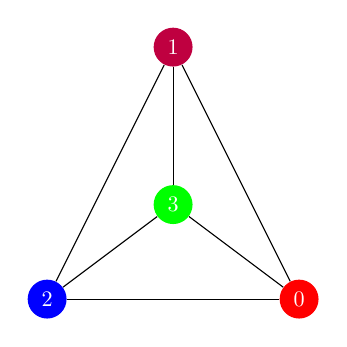
\begin{tikzpicture}[round/.style={circle, text=white, thin, minimum size=.5mm}, transform shape, scale=0.80]
			\node[round, fill=blue] (a) at (0,0){2};
			\node[round, fill=red] (b) at (4,0){0};
			\node[round, fill=green] (c) at (2,1.5){3};
			\node[round, fill=purple] (d) at (2,4){1};
			\draw (a) edge (b);
			\draw (a) edge (c);
			\draw (a) edge (d);
			\draw (b) edge (c);
			\draw (b) edge (d);
			\draw (c) edge (d);
		\end{tikzpicture}
\end{document}